\documentclass{beamer}
\mode<presentation>
{
  \usetheme{boxes}      
  \usecolortheme{whale} 
  \usefonttheme{serif} 
  \setbeamertemplate{navigation symbols}{}
  \setbeamertemplate{caption}[numbered]
} 
\usepackage{graphicx}
\usepackage{tikz}
\setbeamercovered{highly dynamic}
\newcounter{saveenumi}
\newcommand{\seti}{\setcounter{saveenumi}{\value{enumi}}}
\newcommand{\conti}{\setcounter{enumi}{\value{saveenumi}}}
\renewcommand{\thefigure}{\thesection-\arabic{figure}}
\usetikzlibrary{shapes.geometric,calc,angles,positioning,intersections,quotes,decorations,babel,patterns,fit}
\usepackage{tkz-euclide}
\usetkzobj{all}
\usepackage[english]{babel}
\usepackage[utf8]{inputenc}
\usepackage[T1]{fontenc}
\usepackage{graphics}

\usepackage{epstopdf}
\usepackage{standalone}
\usepackage{gensymb}
\usepackage{tikz}
\usetikzlibrary{shapes.geometric,calc,angles,positioning,intersections,quotes,decorations,babel,patterns,fit}
\usepackage{tkz-euclide}
\usetkzobj{all}

\usepackage{amsmath}
\title[Your Short Title]{Exercises}
\author{Durga Prasad}
\institute{}
\date{22 December 2019}
\begin{document}
\begin{frame}
  \titlepage
\end{frame}
\begin{frame}{Triangle exercise}
\begin{enumerate}
\item ABC and AMP are two right triangles, right angled at B and M respectively. M lies on AC and AB is extended to meet P. Prove that:
\seti
\begin{enumerate}
\item $\triangle{ABC} \sim \triangle{AMP}$
\item $\frac{CA}{PA}=\frac{BC}{MP}$
\end{enumerate}
\end{enumerate}
\textbf{Solution:}
\begin{itemize}
\item Consturct a right triangle ABC with a=4, c=3
\item Direction vector m= A-C
\item Representation of AC $n^T(x-A)=0$ and PM $m^T(x-P)=0$
\end{itemize}
\begin{align}
\begin{pmatrix}
m & n
\end{pmatrix}^T M=\begin{pmatrix}
m^T P\\
n^T A
\end{pmatrix}
\end{align}
\end{frame}
\begin{frame}
\begin{figure}[!ht]
\resizebox{.7\linewidth}{!}
{
\begin{tikzpicture}[scale =2.5,>=stealth,point/.style = {draw, circle, fill = black, inner sep = 1pt},]
\node (C) at (4,3)[point,label=above :$\textbf{C(4,3)}$] {};
\node (A) at (0,0)[point,label=below :$\textbf{A(0,0)}$] {};
\node (B) at (4,0)[point,label=below :$\textbf{B(4,0)}$] {};
\node (P) at (5,0)[point,label=below :$\textbf{P(5,0)}$] {};
\node (M) at (3.2,2.4)[point,label=above :$\textbf{M(3.2,2.4)}$] {};
\draw (A)--node[below] {$\textrm{a=4cm}$}(B);
\draw (B)--node[right] {$\textrm{c=3cm}$}(C);
\draw (C)--node[above right] {$\textrm{b}$}(A);
\draw (P)--(M);
\draw (B)--(P);
\tkzMarkRightAngle[fill=white!45,size=.3,mark=](C,B,A)
\tkzMarkRightAngle[fill=white!45,size=.3,mark=](A,M,P)
\end{tikzpicture}


}
\caption{tikz figure}
\label{fig:foo}
\end{figure}
\end{frame}
\begin{frame}
\begin{figure}[!ht]
\resizebox{.5\linewidth}{!}
{

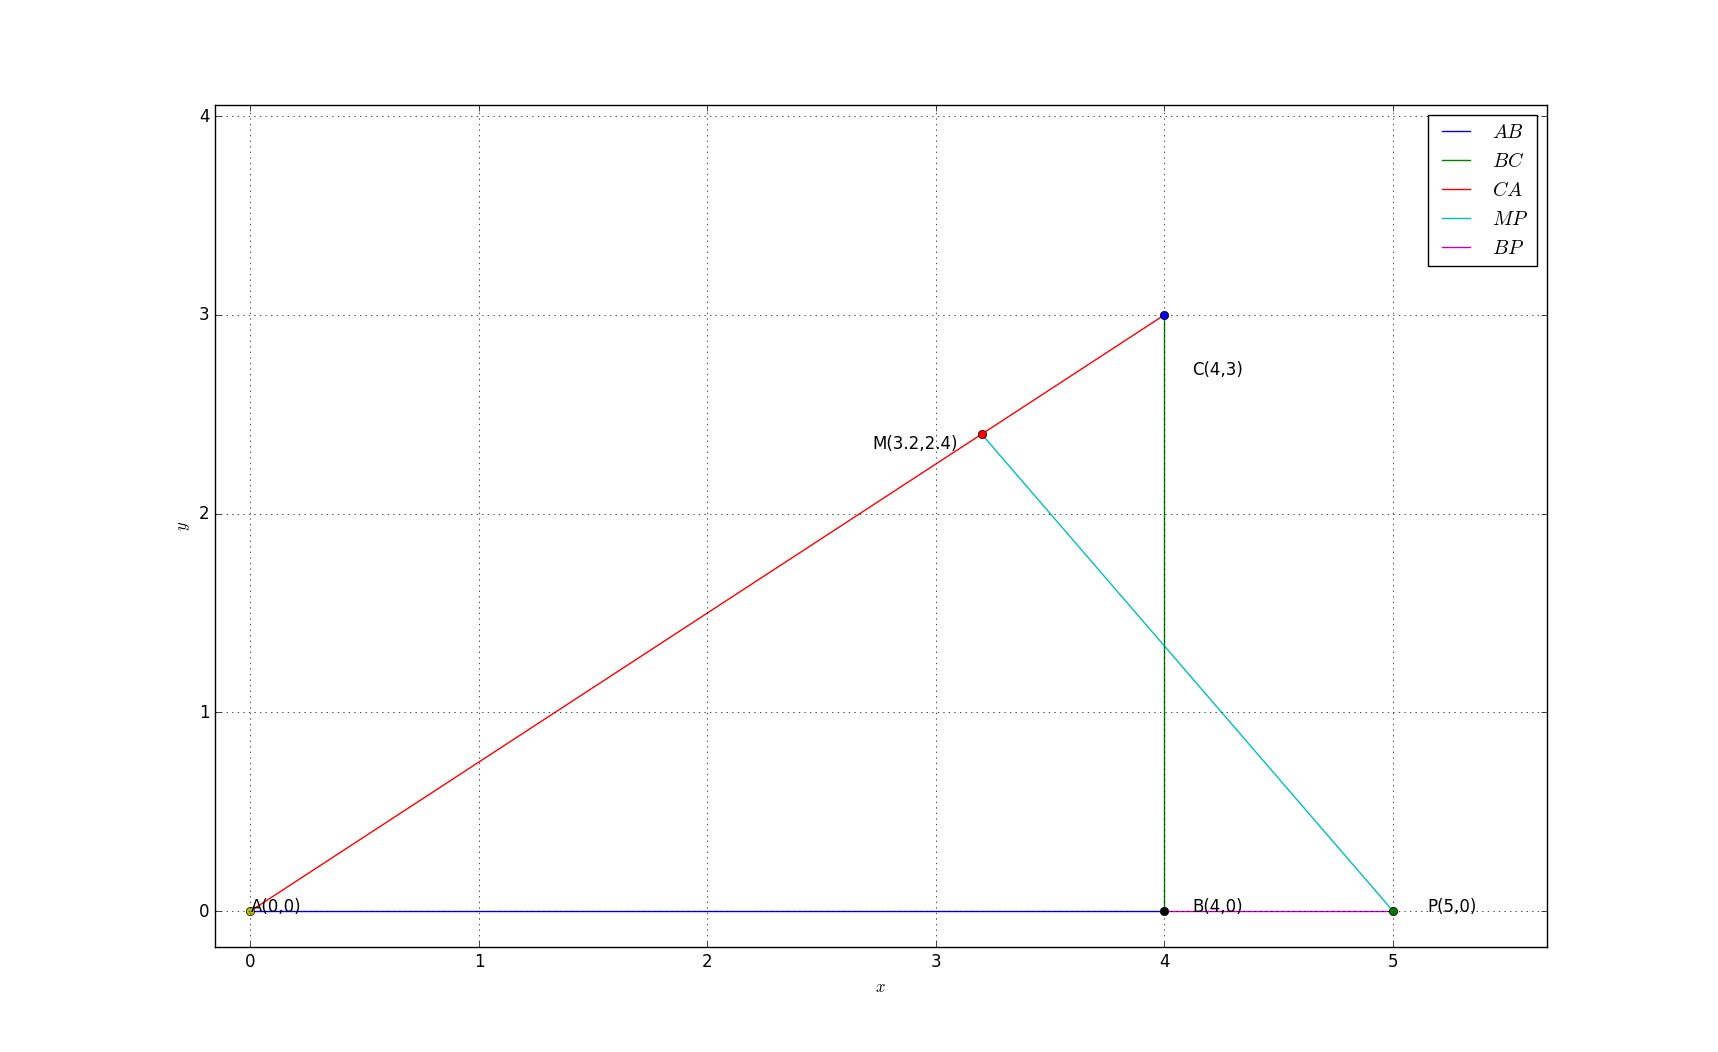
\includegraphics[scale=1.2]{./figs/triangle/tri.png}
}
\caption{Python generated figure}
\label{fig:foo}
\end{figure}
\begin{itemize}
\item \textbf{Python:} \url{https://github.com/d-DP/geometryy/blob/master/codes/triangle/1.tri_exe.py}
\item \textbf{Tkz:} \url{https://github.com/d-DP/geometryy/blob/master/figs/triangle/1.triangle_exercise_fig.tex}
\end{itemize}

\end{frame}
\begin{frame}
From the above figure
\begin{align}
	\angle{CAB} =\angle{MAP} \\
	\angle{ABC} = \angle{AMP}
\end{align}
From 1 and 2
\begin{align}
\triangle{ABC} \sim \triangle{AMP}
\end{align}
\begin{itemize}
\item As correspondinng sides are proportional
$\frac{CA}{PA}=\frac{BC}{MP}=\frac{AB}{AM}$

\begin{center}
$\frac{CA}{PA}=\frac{BC}{MP}$
\end{center}
\end{itemize}

\end{frame}
\begin{frame}{Triangle construction}
\begin{enumerate}
\conti
\item In $\triangle{ABC}$ ,a=8,$\angle{B}=45\degree$ and c-b=3.5. Sketch $\triangle{ABC}$
\seti
\end{enumerate}
\textbf{Solution:}
\begin{figure}[!ht]
\resizebox{0.5\linewidth}{!}
{
\begin{tikzpicture}[scale =1,>=stealth,point/.style = {draw, circle, fill = black, inner sep = 2pt},]
\node (A) at (8.482904196010466,8.482904196010463)[point,label=above :$\textbf{A(8.48,8.48)}$] {};
\node (B) at (0,0)[point,label=above :$\textbf{B(0,0)}$] {};
\node (C) at (8,0)[point,label=below :$\textbf{C(8,0)}$] {};
\draw[->,thick] (A) -- node[above] {$\textbf{c}$} (B) -- node[below] {$\textbf{a=8cm}$} (C) -- node[below,,xshift=1mm] {$\textbf{b}$} (A);
%Drawing and marking angles
\tkzMarkAngle[fill=white!45,size=.3,mark=](C,B,A)
\tkzLabelAngle[pos=0.65](A,B,C){$45$}
\end{tikzpicture}

}
\caption{tikz figure}
\label{fig:foo}
\end{figure}
\end{frame}
\begin{frame}
\begin{figure}[!ht]
\resizebox{1\linewidth}{!}
{
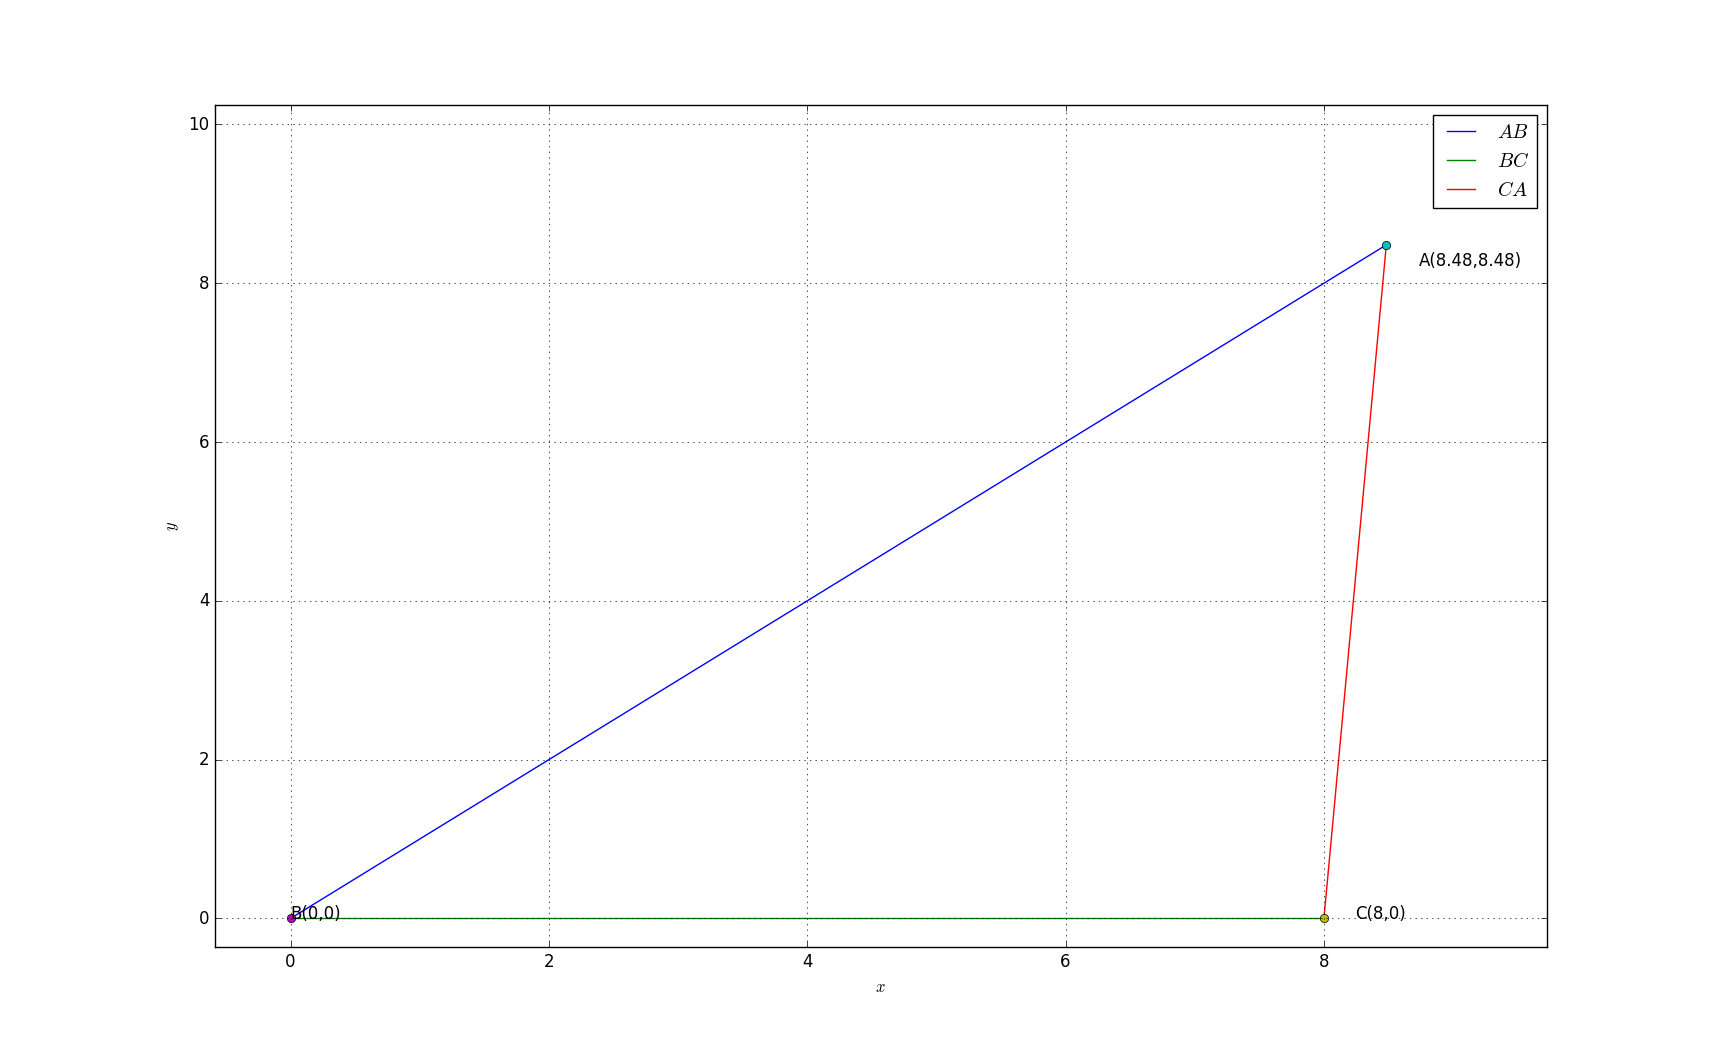
\includegraphics[scale=0.4]{./figs/triangle/constr.png}
}
\caption{Python generated figure}
\label{fig:foo}
\end{figure}
\end{frame}
\begin{frame}
Given a=8cm, c-b=k (k=3.5cm)
Apply cosine rule 
\begin{align*}
	\cos{(B)} = \frac{a^2+c^2-b^2}{2ac}\\
	\cos{(B)}= \frac{a^2+(b+k)^2-b^2}{2a(b+k)}\\
	2ab\cos{B}+2ak\cos{B}=a^2+k+2bk\\
	b=\frac{a^2 + k^2-2ak \cos{B} }{2a\cos{B}-2k}
\end{align*}
\begin{center}
b=8.49, c=11.99
\end{center}
\begin{itemize}
\item \textbf{tikz code:}\url{https://github.com/d-DP/geometryy/blob/master/figs/triangle/2.triangle_construction_fig.tex}\\
\item \textbf{Python code:}\url{https://github.com/d-DP/geometryy/blob/master/codes/triangle/2.tri_constr.py}\\
\end{itemize}
\end{frame}

\begin{frame}{circle constructions}
\begin{enumerate}
\conti 
\item Draw a circle with centre B and radius 6. If C be a point 10 units away from its centre,construct the pair of tangents AC and CD to
the circle.
\seti
\end{enumerate}
\textbf{Solution:}  
\begin{itemize}
\item Draw a circle with radius r=6cm centre B.
\item Apply Baudhayana theorem ABC and BCD to get AC,DC distance and find A and D coordinates.$$B=\begin{pmatrix}
0 \\ 0
\end{pmatrix}
C=\begin{pmatrix}
10 \\ 0
\end{pmatrix} 
A=\begin{pmatrix}4.5\\3.96\end{pmatrix} D=\begin{pmatrix}4.5\\-3.96\end{pmatrix}$$

\end{itemize}
\end{frame}
\begin{frame}
\begin{figure}[!ht]
\resizebox{0.8\linewidth}{!}
{
\begin{tikzpicture}[scale =1.5,>=stealth,point/.style = {draw, circle, fill = black, inner sep = 1pt},]
\draw (0,0)circle (6cm);
\node (C) at (10,0)[point,label=above :$\textbf{C(10,0)}$] {};
\node (A) at (4.5,3.96862697)[point,label=below :$\textbf{A(4.5,3.96)}$] {};
\node (B) at (0,0)[point,label=below :$\textbf{B(0,0)}$] {};
\node (D) at (4.5,-3.96862697)[point,label=below :$\textbf{D(4.5,-3.96)}$] {};
\draw (B)--node[below] {$\textbf{10cm}$}(C)--(D)--(B);
\draw (B)--(A)--(C);
\end{tikzpicture}



}
\caption{Circle with tikz}
\label{fig:foo}
\end{figure}
\end{frame}
\begin{frame}
\begin{figure}[!ht]
\resizebox{0.5\linewidth}{!}
{
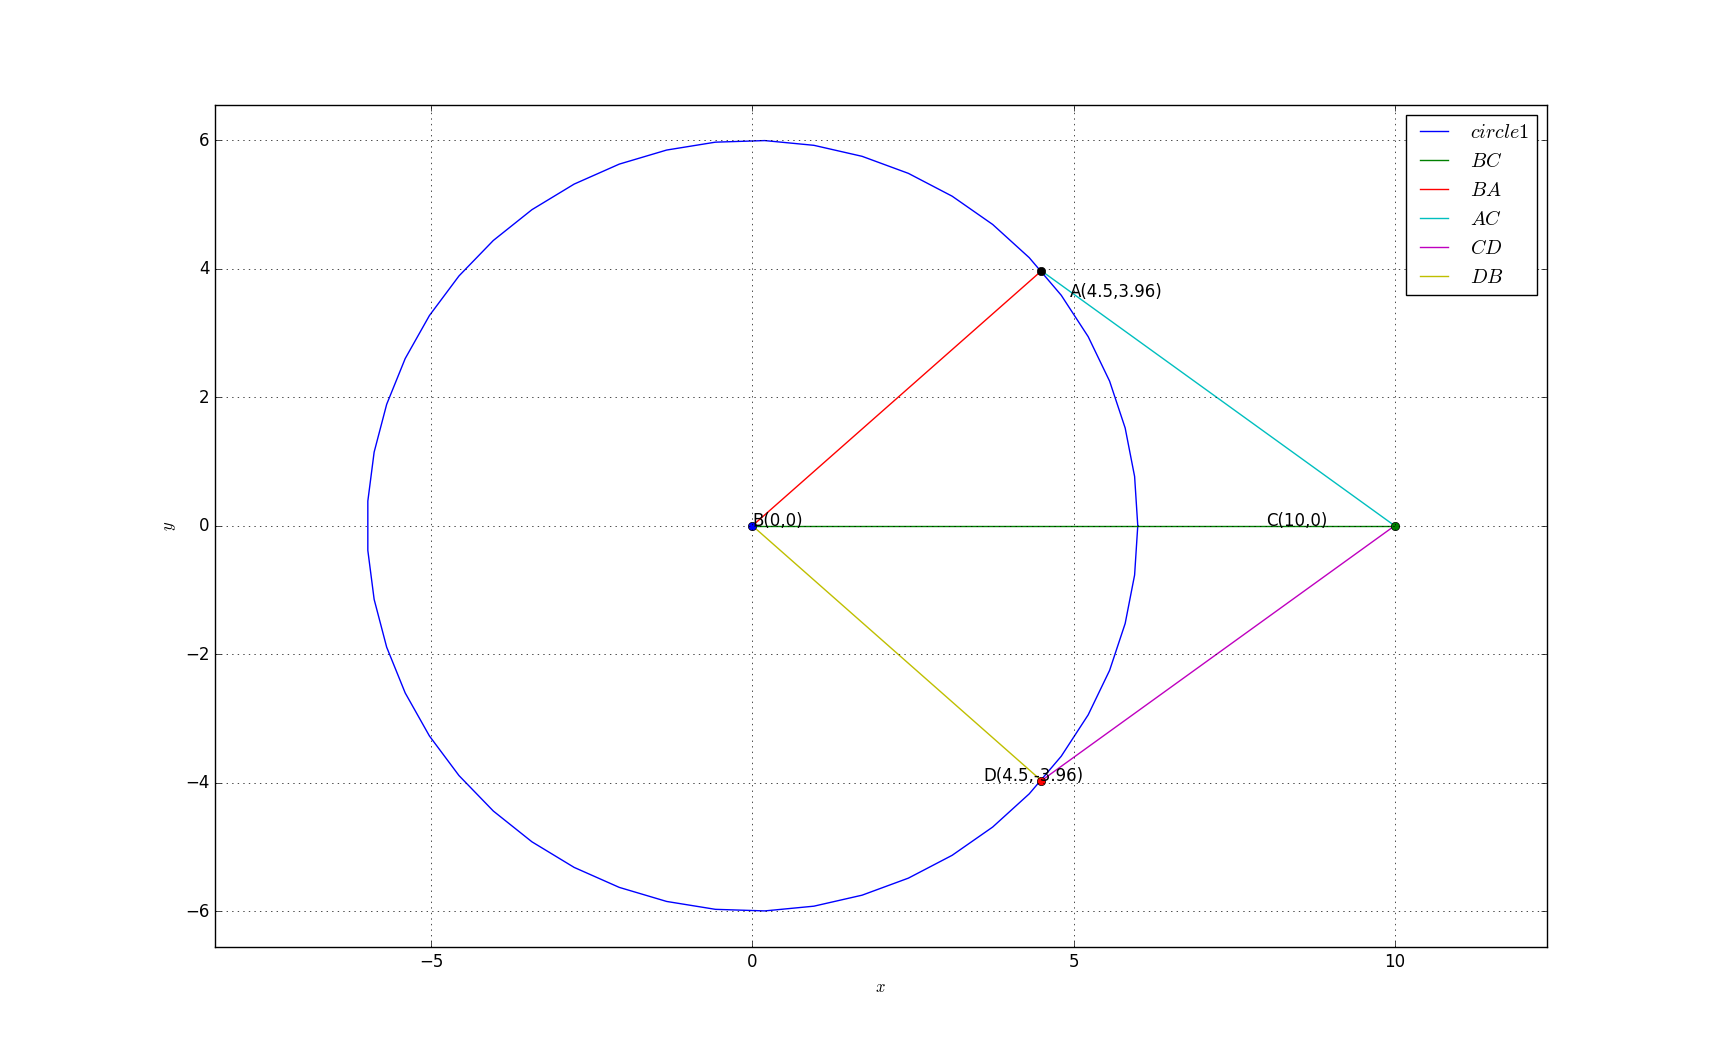
\includegraphics[scale=1.5]{./figs/circles/circle_constr.png}
}
\caption{Circle with python}
\label{fig:foo}
\end{figure}
\begin{itemize}
\item \textbf{python code :}\url{https://github.com/d-DP/geometryy/blob/master/codes/circles/circle_constr.py}\\
\item \textbf{tikz :}\url{https://github.com/d-DP/geometryy/blob/master/figs/circles/circle_constr.tex}
\end{itemize}
\end{frame}
\begin{frame}{Miscellaneous}
\begin{enumerate}
\conti
\item The lengths of two parallel chords of a circle are 6 cm and 8 cm. If the smaller chord is
at distance 4 cm from the centre, what is the
distance of the other chord from the centre?
\seti
\end{enumerate}
\textbf{Solution:} 
\begin{figure}[!ht]
\resizebox{0.45\linewidth}{!}
{
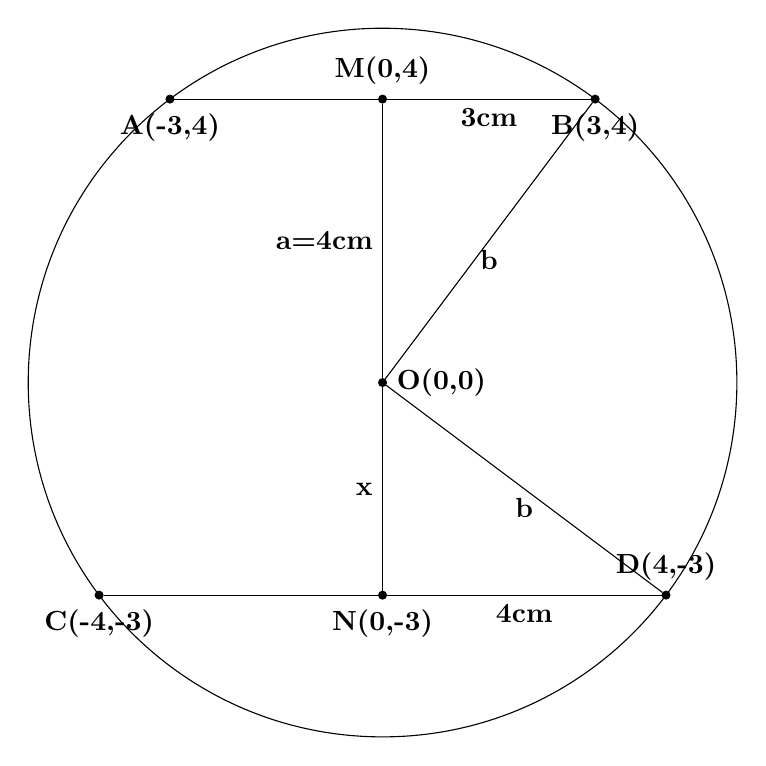
\begin{tikzpicture}[scale =0.9,>=stealth,point/.style = {draw, circle, fill = black, inner sep = 1pt},]
\draw (0,0)circle (5cm);
\node (O) at (0,0)[point,label=right :$\textbf{O(0,0)}$] {};
\node (A) at (-3,4)[point,label=below :$\textbf{A(-3,4)}$] {};
\node (B) at (3,4)[point,label=below :$\textbf{B(3,4)}$] {};
\node (C) at (-4,-3)[point,label=below :$\textbf{C(-4,-3)}$] {};
\node (D) at (4,-3)[point,label=above :$\textbf{D(4,-3)}$] {};
\node (M) at (0,4)[point,label=above :$\textbf{M(0,4)}$] {};
\node (N) at (0,-3)[point,label=below :$\textbf{N(0,-3)}$] {};
\draw (A)--(B);
\draw (C)--(D);
\draw (O)--node[left] {$\textbf{a=4cm}$}(M);
\draw (O)--node[left] {$\textbf{x}$}(N);
\draw (O)--node[below] {$\textbf{b}$}(B);
\draw (O)--node[below] {$\textbf{b}$}(D);
\draw (M)--node[below] {$\textbf{3cm}$}(B);
\draw (N)--node[below] {$\textbf{4cm}$}(D);
\end{tikzpicture}

}
\caption{tikz figure}
\label{fig:foo}
\end{figure}
\end{frame}
\begin{frame}
\begin{figure}[!ht]
\resizebox{0.45\linewidth}{!}
{
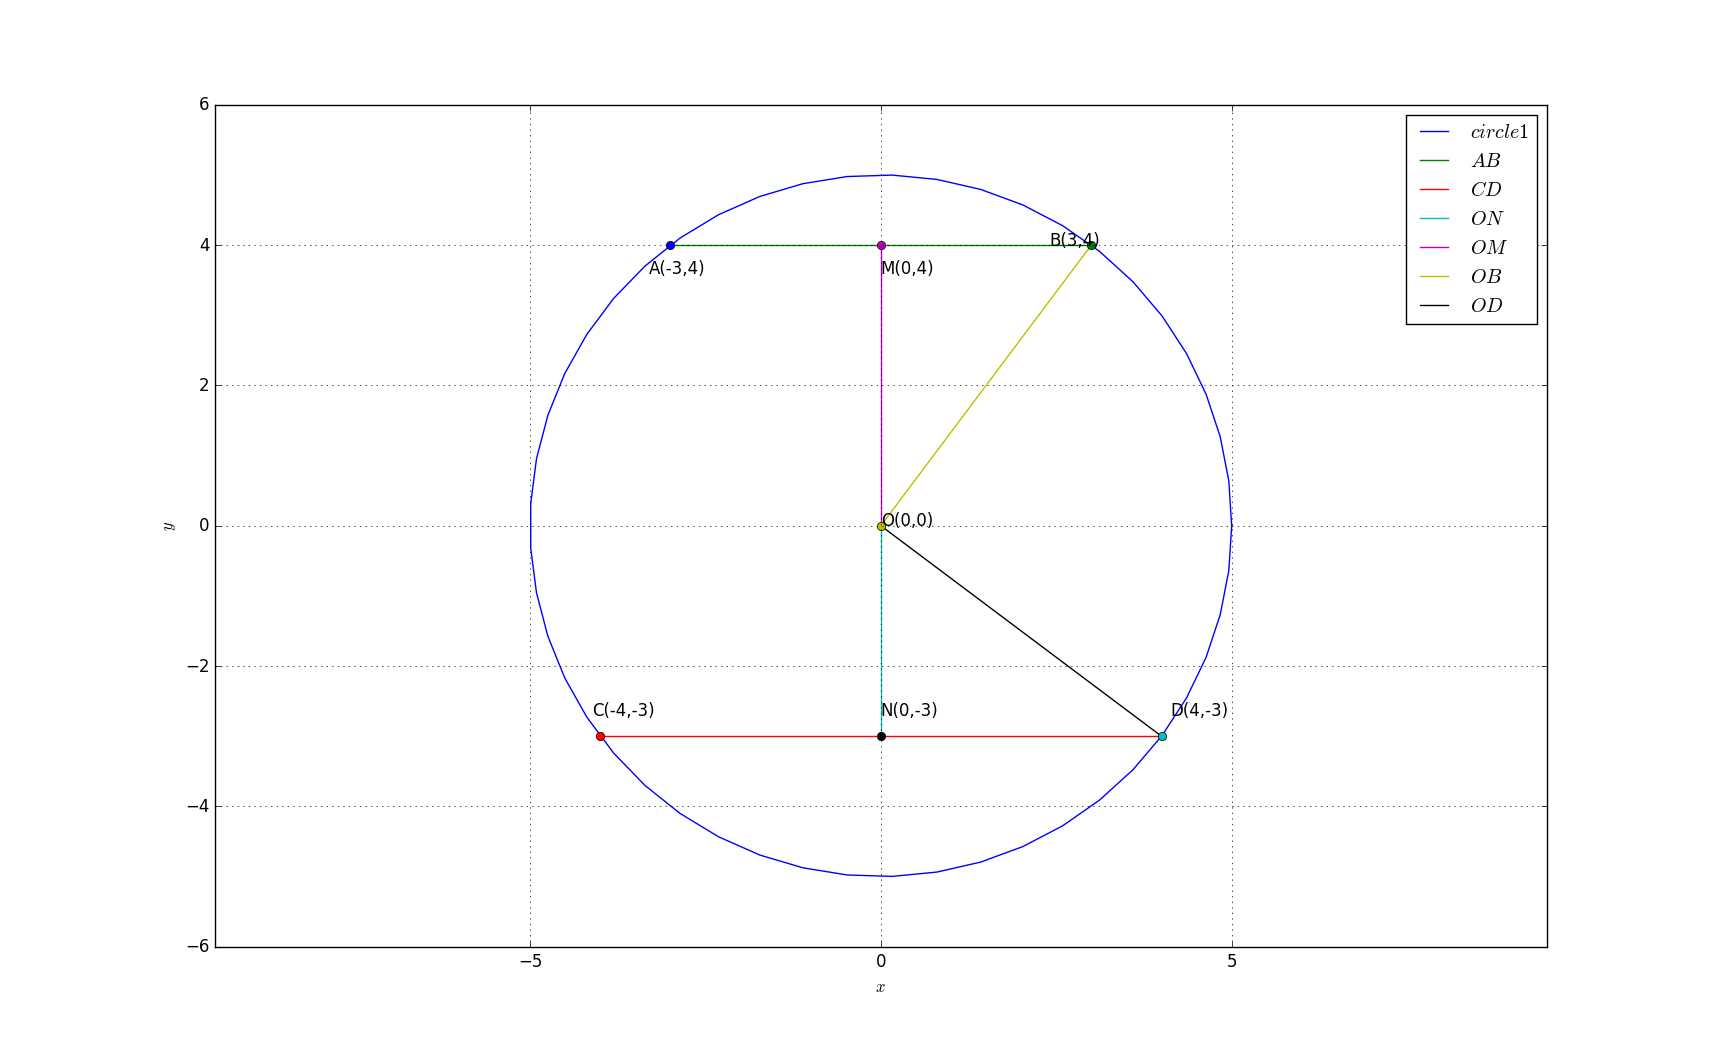
\includegraphics[scale=1.2]{./figs/misc.png}
}
\caption{Python generated figure}
\label{fig:foo}
\end{figure}
Apply Baudhayana theorem for $\triangle{MOB}$ and $\triangle{NOD}$
\begin{align*}
a^2+(3)^2=(b)^2 \\
x^2+(4)^2=b^2
\end{align*}
\begin{itemize}
\item \textbf{python:} \url{https://github.com/d-DP/geometryy/blob/master/codes/misc.py}
\item \textbf{tikz:} \url{https://github.com/d-DP/geometryy/blob/master/figs/misc.tex}
\end{itemize}
\end{frame}
\begin{frame}{Quadrilateral construction}
\begin{enumerate}
\conti
\item construct a quadrilateral MIST where MI =3.5, IS = 6.5, $\angle{M}= 75\degree,\angle{I}=105\degree$ and $\angle{s}=120\degree$
\seti
\end{enumerate}
\textbf{Solution:}
\begin{itemize}
\item Given that MI=8 and IS=6.5 Apply cosine law for $\triangle{MIS}$
\begin{align*}
c=\sqrt{a^{2}+b^{2}-2ab \times \cos\angle{M}}
\end{align*}
\item Find S coordinates
\begin{itemize}
\item Directon vector for ST is $$m1=\begin{pmatrix}
1 \\ \tan{135\degree}
\end{pmatrix}$$
\item Normal vector for MT is
\begin{align}
n_1^T T=n_1^T S
\end{align}
\item Direction vector for ST=MT,m2=S-I
\item Normal vector 
\begin{align}
n_2^T{T}=0
\end{align}


\end{itemize}
\end{itemize}
\end{frame}
\begin{frame}
\begin{align}
\begin{pmatrix} n_1 \\ n_2 \end{pmatrix}^T T=\begin{pmatrix}
n_1^T S \\ n_2^T M
\end{pmatrix}
\end{align}
\begin{figure}[!h]
\resizebox{0.4\linewidth}{!}
{
\begin{tikzpicture}[scale =2.5,>=stealth,point/.style = {draw, circle, fill = black, inner sep = 2pt},]
\node (M) at (0,0)[point,label=below right :$\textbf{M(0,0)}$] {};
\node (I) at (3.5,0)[point,label=below right :$\textbf{I(3.5,0)}$] {};

\node (S) at (5.18232379,6.27851787)[point,label=above right :$\textbf{S(5.18,6.27)}$] {};
\node (T) at (2.42196082,9.03888084)[point,label=above :$\textbf{T(2.42,9.03)}$] {};
\draw (M) --node[below ] {$\textbf{a=3.5cm}$}(I)--node[below ] {$\textbf{b	=3.5cm}$}(S)--(T)--(M);
\draw (M) --node[below ] {$\textbf{c=3.5cm}$}(S);
\tkzMarkAngle[fill=black!45,size=.3,mark=](I,M,S)
\tkzLabelAngle[pos=0.65](I,M,S){}
\tkzMarkAngle[fill=black!45,size=.3,mark=](S,M,T)
\tkzLabelAngle[pos=0.65](S,M,T){$75\degree$}
\tkzMarkAngle[fill=black!45,size=.3,mark=](S,I,M)
\tkzLabelAngle[pos=0.65](S,I,M){$105\degree$}

\tkzMarkAngle[fill=black!45,size=.3,mark=](T,S,I)
\tkzLabelAngle[pos=0.65](T,S,I){$120\degree$}
\tkzMarkAngle[fill=black!45,size=.3,mark=](M,T,S)
\tkzLabelAngle[pos=0.65](M,T,S){$75\degree$}
\end{tikzpicture}

}
\caption{Quadrilateral with tikz}
\label{fig:foo}
\end{figure}
\end{frame}
\begin{frame}
\begin{figure}[!h]
\resizebox{0.9\linewidth}{!}
{
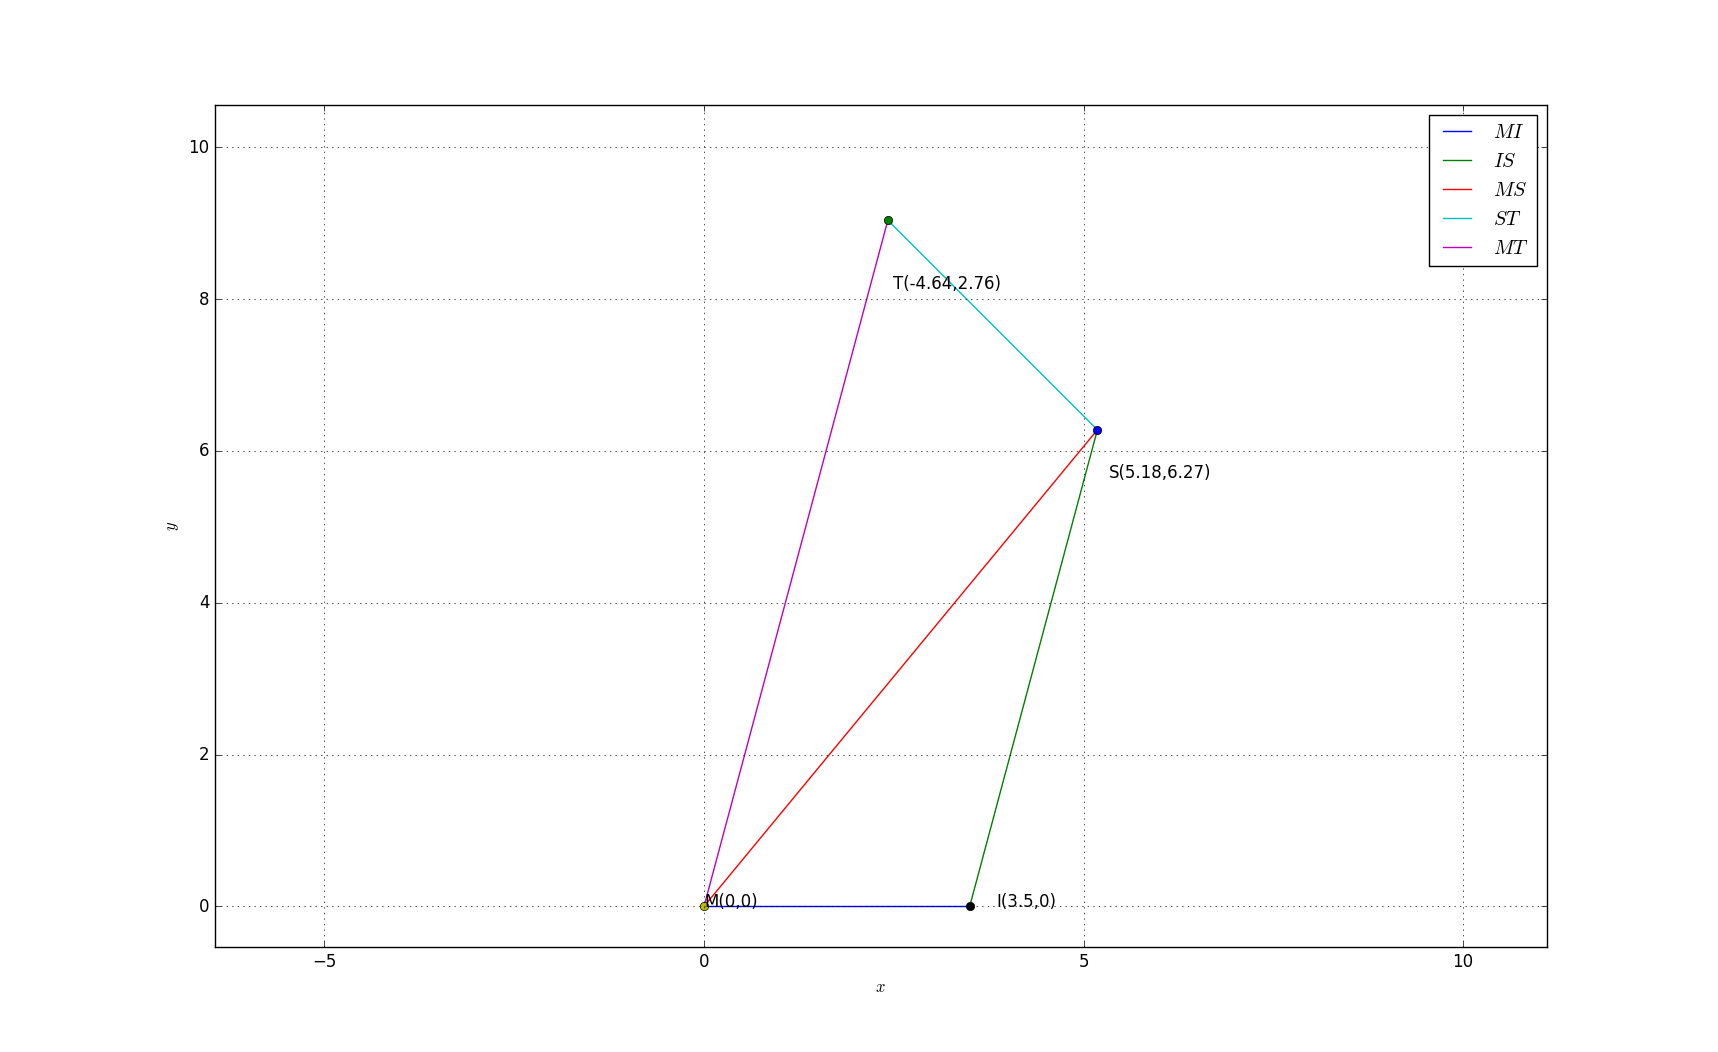
\includegraphics[scale=0.4]{./figs/quad/quad_constr1.png}
}
\caption{Quadrilateral with python}
\label{fig:foo}
\end{figure}
\begin{itemize}
\item \textbf{python :}\url{https://github.com/d-DP/geometryy/blob/master/codes/quad/quad_constr1.py}\\
\item \textbf{tikz:} \url{https://github.com/d-DP/geometryy/blob/master/figs/quad/quad_constr.tex}
\end{itemize}
\end{frame}

\begin{frame}{Circle Exercise}
\begin{enumerate}
\conti
\item Two circles intersect at two points B and C.
Through B, two line segments ABD and PBQ
are drawn to intersect the circles at A, D and
P, Q respectively. Prove that $\angle{ACP}=\angle{QCD}$
\seti
\end{enumerate}
\textbf{Solution:}
\begin{align*}
||x||^2 =r^2\\
P=B+\lambda{m}\\
x=B+\lambda{m}\\
||B+\lambda m||^2 = r^2\\
(B+\lambda m)^T(B+\lambda m) =r^2\\
\lambda ^2||m||^2 +2\lambda m^T B=r^2
\end{align*}
\end{frame}
\begin{frame}
\begin{figure}[!ht]
\resizebox{0.6\linewidth}{!}
{
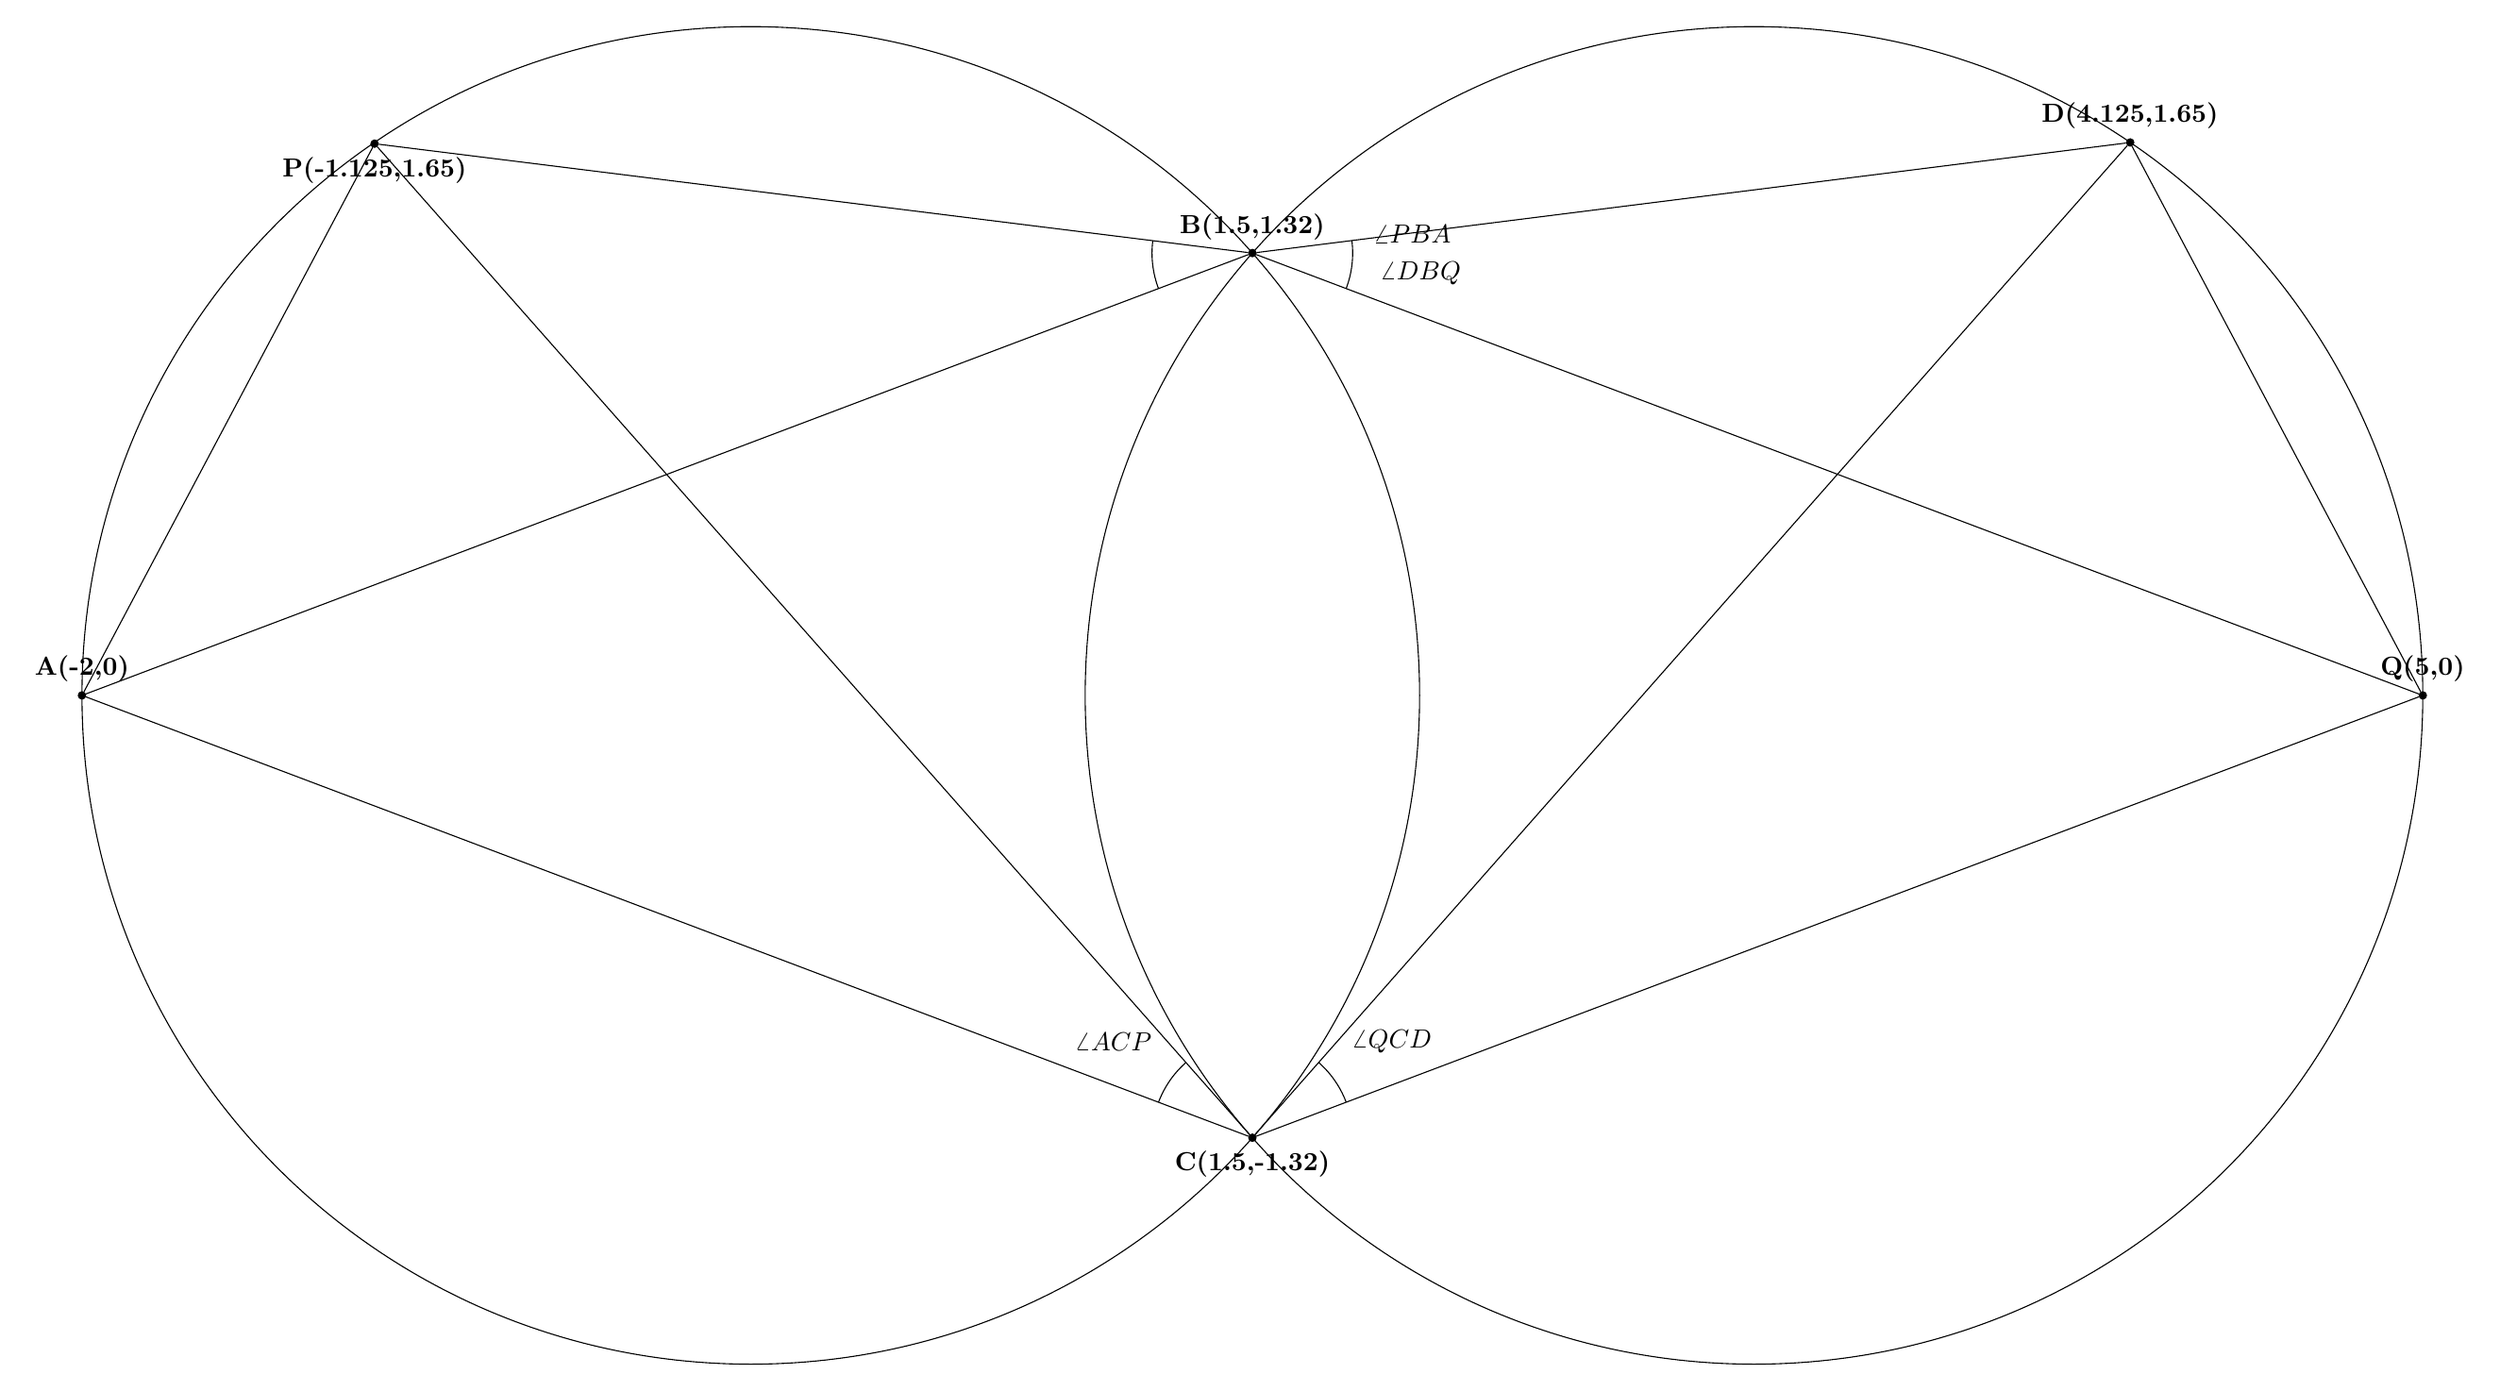
\begin{tikzpicture}[scale =4.5,>=stealth,point/.style = {draw, circle, fill = black, inner sep = 1pt},]
\draw (0,0)circle (2cm)(3,0) circle (2cm);
\node (A) at (-2,0)[point,label=above :$\textbf{A(-2,0)}$] {};
\node (P) at (-1.125,1.65)[point,label=below :$\textbf{P(-1.125,1.65)}$] {};
\node (B) at (1.5,1.3228756555322954)[point,label=above :$\textbf{B(1.5,1.32)}$] {};
\node (Q) at (5,0)[point,label=above :$\textbf{Q(5,0)}$] {};
\node (D) at (4.125,1.65359457)[point,label=above :$\textbf{D(4.125,1.65)}$] {};
\node (C) at (1.5,-1.3228756555322954)[point,label=below :$\textbf{C(1.5,-1.32)}$] {};
\draw (A)--(P)--(B)--(Q)--(C)--(P);
\draw (A)--(B)--(D)--(C)--(A);
\draw (D)--(Q);
\tkzMarkAngle[fill=black!45,size=.3,mark=](P,B,A)
\tkzLabelAngle[pos=-0.5](P,B,A){$\angle{PBA}$}
\tkzMarkAngle[fill=black!45,size=.3,mark=](P,C,A)
\tkzLabelAngle[pos=0.5](P,C,A){$\angle{ACP}$}

\tkzMarkAngle[fill=green!45,size=.3,mark=](Q,B,D)
\tkzLabelAngle[pos=0.5](Q,B,D){$\angle{DBQ}$}
\tkzMarkAngle[fill=green!45,size=.3,mark=](Q,C,D)
\tkzLabelAngle[pos=0.5](Q,C,D){$\angle{QCD}$}
\end{tikzpicture}



}
\caption{Circle tikz}
\label{fig:foo}
\end{figure}
\end{frame}
\begin{frame}
\begin{figure}[!ht]
\resizebox{0.6\linewidth}{!}
{
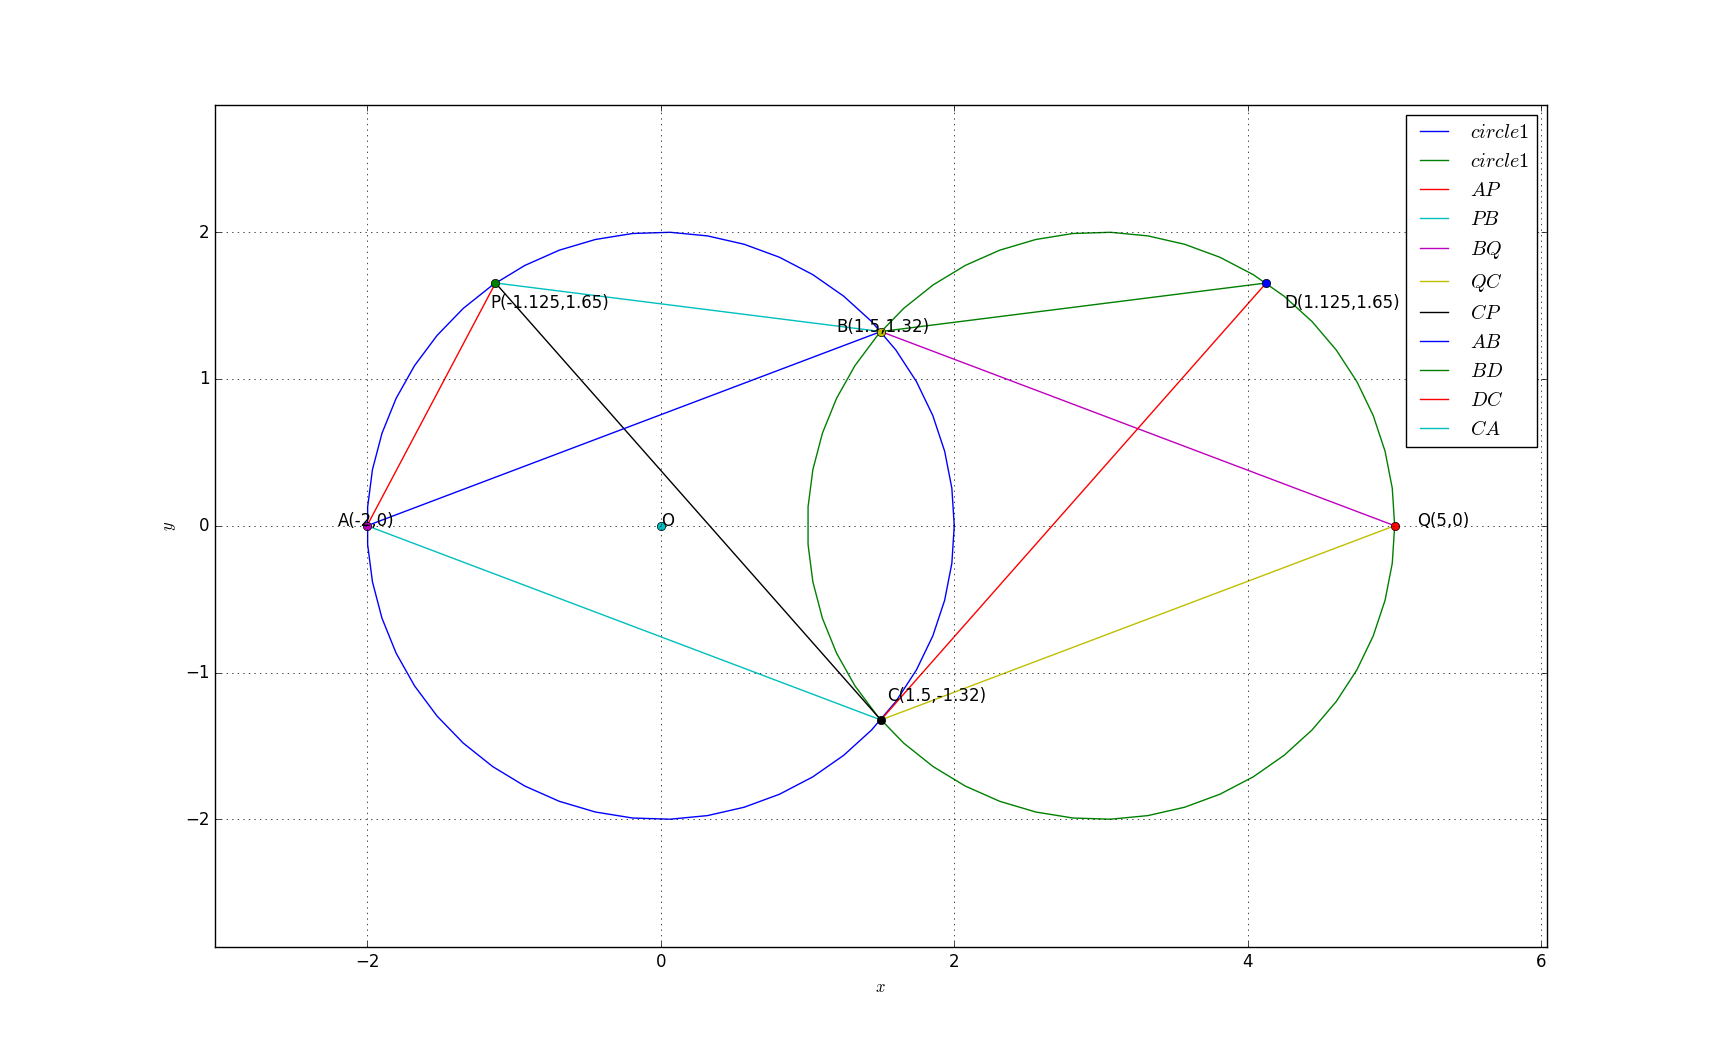
\includegraphics[scale=1.2]{./figs/circles/3.png}
}
\caption{Python figure}
\label{fig:foo}
\end{figure}
\end{frame}
\begin{frame}
From the above figure
\begin{align}
\angle{PBA}=\angle{ACP}\\
\angle{DBQ}=\angle{QCD}\\
\angle{PBA}=\angle{DBQ}
\end{align}
from 10,11,12 $\angle{ACP}=\angle{QCD}$\\
\begin{itemize}
\item \textbf{python code :} \url{https://github.com/d-DP/geometryy/blob/master/codes/circles/3.py}\\
\item \textbf{tikz:}\url{https://github.com/d-DP/geometryy/blob/master/figs/quad/quad_exer.tex}
\end{itemize}
\end{frame}
\begin{frame}{Quadrilateral exercise}
\begin{enumerate}
\conti
\item ABCD is a rhombus and P, Q, R and S are the
mid-points of the sides AB, BC, CD and DA
respectively. Show that the quadrilateral PQRS
is a rectangle.
\seti
\end{enumerate}
\textbf{Solution:}
\begin{itemize}
\item Construct a rhombus wih following coordinates $$A=\begin{pmatrix}
0 \\3 
\end{pmatrix},
B=\begin{pmatrix}
5 \\0 
\end{pmatrix},
C=\begin{pmatrix}
0 \\3
\end{pmatrix},
D=\begin{pmatrix}
-5 \\0 
\end{pmatrix}$$
\item Find P,Q,R,S
\item $P=\frac{(A+D)}{2},Q=\frac{(D+C)}{2},R=\frac{(C+B)}{2} and S=\frac{(A+B)}{2}$
\end{itemize}
\end{frame}
\begin{frame}
\begin{figure}[!h]
\resizebox{0.5\linewidth}{!}
{
\begin{tikzpicture}[scale =2.5,>=stealth,point/.style = {draw, circle, fill = black, inner sep = 2pt},]
\node (A) at (0,-3)[point,label=below :$\textbf{A(0,-3)}$] {};
\node (B) at (5,0)[point,label=above :$\textbf{B(5,0)}$] {};
\node (D) at (-5,0)[point,label=below :$\textbf{D(-5,0)}$] {};
\node (C) at (0,3)[point,label=above :$\textbf{C(0,3)}$] {};
\node (S) at (-2.5,-1.5)[point,label=above left :$\textbf{S(-2.5,-1.5)}$] {};
\node (R) at (-2.5,1.5)[point,label=above left :$\textbf{R(-2.5,1.5)}$] {};
\node (Q) at (2.5,1.5)[point,label=above right :$\textbf{Q(2.5,1.5)}$] {};
\node (P) at (2.5,-1.5)[point,label=below right :$\textbf{P(2.5,-1.5)}$] {};
\draw (A) --(B)--(C)--(D)--(A);
\draw (P) --(Q)--(R)--(S)--(P);
\draw (Q) --(S);
\draw (P) --(R);
\draw (A) --(C);
\draw (B) --(D);
\tkzMarkAngle[fill=black!45,size=.3,mark=](S,P,A)
\tkzLabelAngle[pos=-0.55](S,P,A){$\angle{3}$}
\tkzMarkAngle[fill=blue!45,size=.3,mark=](B,P,Q)
\tkzLabelAngle[pos=0.45](B,P,Q){$\angle{1}$}
\tkzMarkAngle[fill=red!45,size=.3,mark=](P,Q,B)
\tkzLabelAngle[pos=0.45](P,Q,B){$\angle{2}$}
\tkzMarkAngle[fill=green!45,size=.3,mark=](C,Q,R)
\tkzLabelAngle[pos=0.45](C,Q,R){$\angle{4}$}
\end{tikzpicture}


}
\caption{tikz figure}
\label{fig:foo}
\end{figure}
\end{frame}
\begin{frame}
\begin{figure}[!h]
\resizebox{0.3\linewidth}{!}
{
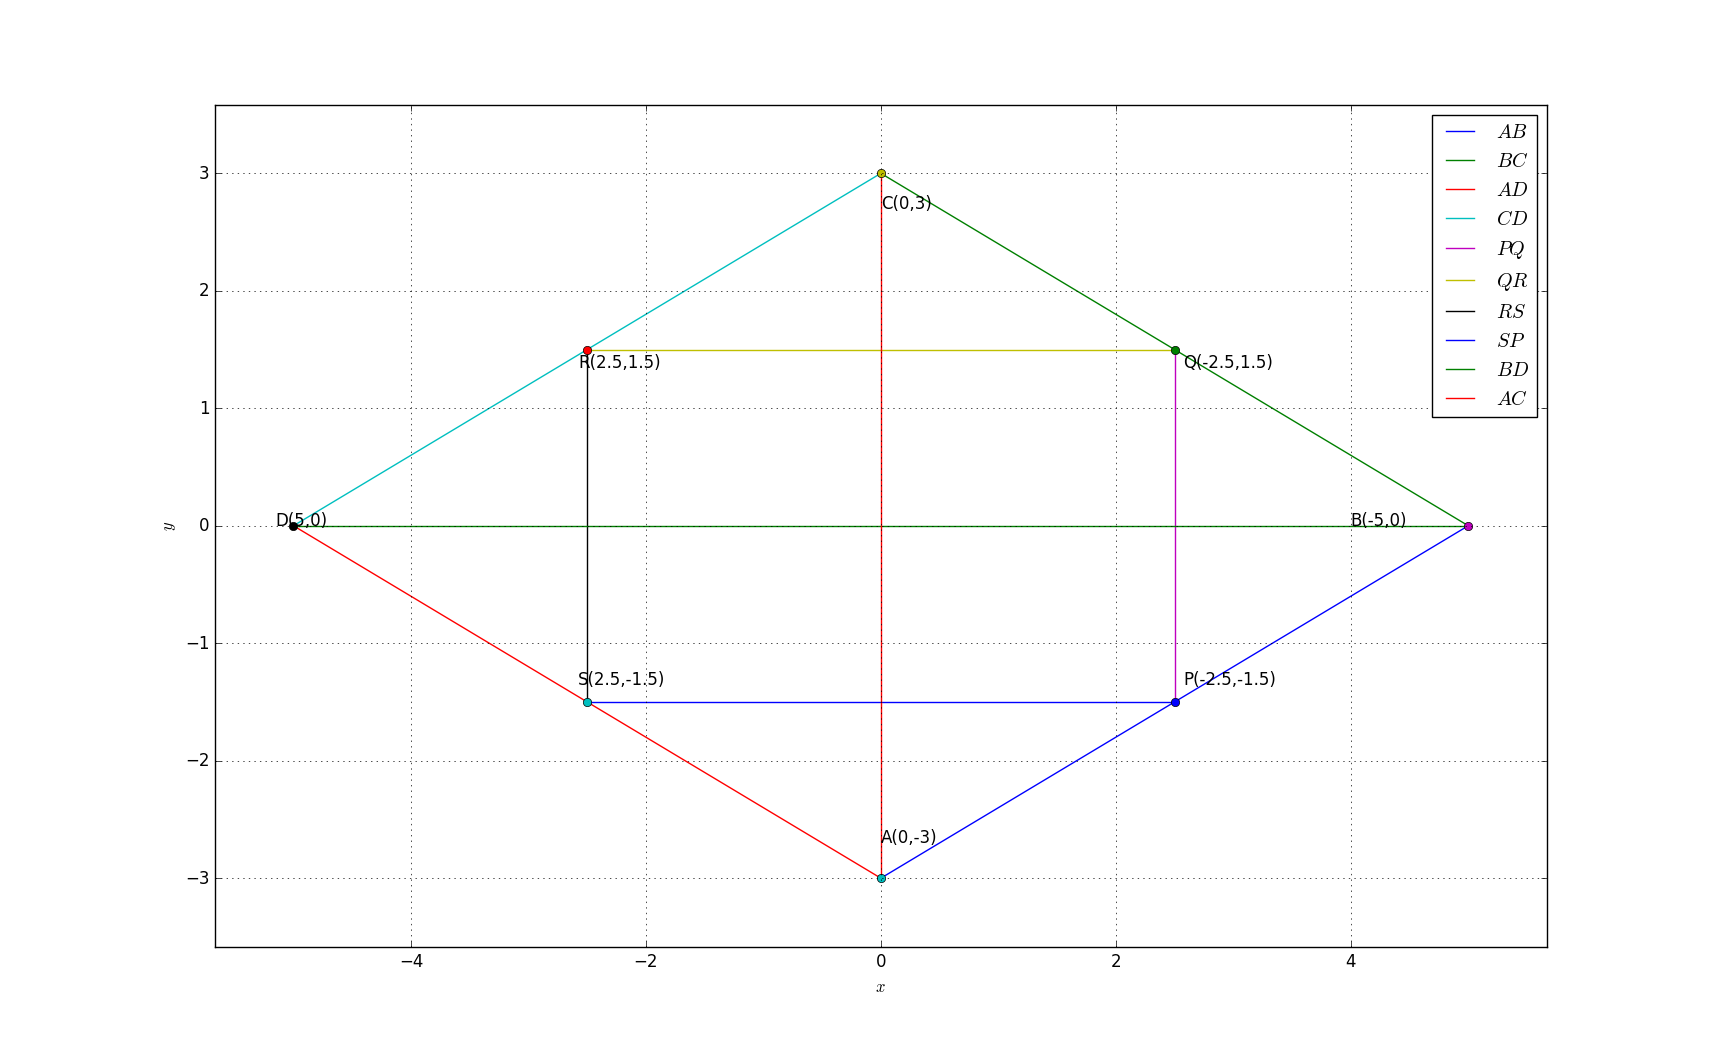
\includegraphics[scale=1.2]{./figs/quad/rhomb.png}

}
\caption{Rhombus}
\label{fig:foo}
\end{figure}
From $\triangle{ABC}$ and $\triangle{ADC}$
\begin{align}
PQ || AC \hspace{2pt}\text{and}\hspace{2pt} PQ=\frac{1}{2}AC\\
RS || AC \hspace{2pt}\text{and}\hspace{2pt} RS=\frac{1}{2}AC
\end{align}
from 11 and 12 PQ=RS , PQ||RS 
\begin{align}
 \textit{As}\hspace{6pt} PB=PQ, \angle{2} =\angle{1}
\end{align}
From $\triangle{APS}$ and $\triangle{CQR}$ \\
\begin{itemize}
\item AP=CQ,AS=CR, PS=QR\\
\item From SSS rule
$\triangle{APS} \cong \triangle{CQR}$
\begin{align}
\angle{3} = \angle{4}
\end{align}
\end{itemize}
\end{frame}
\begin{frame}
For AB, BC
\begin{align}
\angle{3}+\angle{SPQ}+\angle{1} = 180\degree
\end{align}
\begin{align*}
\angle{2}+\angle{PQR}+\angle{4}=180\degree
\end{align*}
from 13 and 15 
\begin{align}
\angle{1}+\angle{PQR}+\angle{3}=180\degree
\end{align}
\begin{center}
PS|| PR $\angle{SPQ}+\angle{PQR} =180\degree \implies \angle{SPQ}=90\degree$
\end{center}
tikz : \url{https://github.com/d-DP/geometryy/blob/master/figs/quad/quad_exer.tex}\\
python : \url{https://github.com/d-DP/geometryy/blob/master/codes/quad/rhombus.py}
\end{frame}
\end{document}